
\section{倫理ある商取引ゲーム}
% 「不正防止の不可能性」より,「商取引ゲーム」においては不正を防止するインセンティブ設計ができないことがわかった.しかし,この理論上の商取引に反して,実社会の商取引においては不正行為がある程度抑制されている.これは実社会の商取引を行う人々が,自身の利益を最大化するような利己的な行動規範に従って戦略を選んでおらず,完全な「商取引ゲーム」を行っていないためだからだと考えられる.そこで本稿では,この利己的でない行動規範を「倫理」とし,「倫理」に従うプレイヤーのみで行われる「商取引ゲーム」を「倫理ある商取引ゲーム」とすることで,この「倫理ある商取引ゲーム」において不正を防止するインセンティブ設計が可能であることを示す.

\subsection{倫理}
「不正防止の不可能性」より,「商取引ゲーム」においては不正を防止するインセンティブ設計ができないことがわかった.しかし,この理論上の商取引に反して,実社会の商取引においては不正行為がある程度、抑制されている.これは実社会の商取引を行う人々が,自身の利益を最大化するような利己的な行動規範に従って戦略を選んでおらず,完全な「商取引ゲーム」を行っていないためだと考えられる.本稿では、実社会の商取引において「泣き寝入り」と呼ばれるような$buyer$が不正にあった場合に「成功」を報告する戦略があまり取られていないことに着目し、$buyer$が不正にあった場合に必ず「失敗」を報告する行動規範を倫理として定義し、この倫理に従うプレイヤーのみで行われる「商取引ゲーム」を「倫理ある商取引ゲーム」とする.

% 「不正防止の不可能性」より,「商取引ゲーム」においては不正を防止するインセンティブ設計ができないことがわかった.しかし,この理論上の商取引に反して,実社会の商取引においては不正行為がある程度抑制されている.これは実社会の商取引を行う人々が,自身の利益を最大化するような利己的な行動規範に従って戦略を選んでおらず,完全な「商取引ゲーム」を行っていないためだと考えられる.そこで、本稿ではそのような行動規範を倫理と定義し、利己的な行動規範との違いについて論じる.

% 利己的な行動規範とは,相手が各戦略をとる主観的な確率とその際の自身の利得から自身の各戦略の期待利得を算出し,それが高い方の戦略を選択する行動規範である.各利得は「商取引システム」から一意に決定されるため,「倫理」と利己的な行動規範の差異は相手が各戦略をとる主観的な確率にあると考えられる.つまりは相手が特定の戦略をとる確率を通常よりも低く(もしくは高く)見積もっていることになる.そのため倫理が具体的にどのように利己的な行動規範と違うのかを知るためには、$seller$と$buyer$のとりえる各戦略について考える必要がある.
%
% 「商取引ゲーム」においては$seller$の戦略は2通りあり$buyer$の戦略は4通りあった.これらの戦略は「$seller$が商品を渡すか否か」と「$buyer$が商品の受け取りを報告するか否か」,「$buyer$が不正にあった場合に告発するか否か」の3つの観点から2分できる.そこで,それらの観点で2分した片方の戦略群を相手が選ぶ可能性が0であるとした場合について考える.また,この主観的な確率が0であるとみなす戦略をそのプレイヤーはとりえないものとして考える.本稿では、実社会の商取引において「泣き寝入り」と呼ばれるような戦略があまり取られていないことに着目し、$buyer$が不正にあった場合に必ず「失敗」を報告する行動規範を倫理として定義する.

\subsection{倫理ある商取引ゲーム}
「倫理ある商取引ゲーム」においては$buyer$は$seller$が不正を行った場合にかならず「失敗」を報告するためゲーム木はFigure\ref{ethical-gametree}のようになる.また、同様に$buyer$が戦略$s^{buyer}_2, s^{buyer}_4$を取らないため、非協力戦略型ゲームの表はTable\ref{ethical-gametable}のようになる.


% まず「$seller$が商品を渡すか否か」について考察する.プレイヤーが$seller$の「商品を渡す」という戦略を取りえない行動規範に従って戦略を選ぶとき「商取引ゲーム」は必ず失敗する.また,プレイヤーが「商品を渡さない」という戦略を取り得ない行動規範に従って戦略を選ぶとき,「商取引ゲーム」を成功させるインセンティブ設計は可能になるが,これは「プレイヤーが不正を起こさないから成功する」というようなものである.
% 次に「$seller$が商取引契約を履行した場合に$buyer$が『成功』を報告するか否か」については,$buyer$が「$seller$が履行した場合に『失敗』を報告する」戦略をとる「商取引ゲーム」では誠実な戦略組をとり得ることはなく,$buyer$が「$seller$が商取引契約を履行した場合に『成功』を報告する」戦略をとるなら,必ず$seller$は商取引契約を反故にするだろう.
% 最後に「$seller$が商取引契約を反故にした場合に$buyer$が『成功』を報告するか否か」について,$buyer$が$seller$が商取引契約を反故にした場合に必ず『成功』を報告するなら,$seller$は必ず商取引契約を反故にするだろう.残るは「$seller$が商取引契約を反故にした場合に必ず『失敗』を報告する」場合である.この場合のときのみ,$seller$は商取引契約を履行するか反故にするかの選択を商品価値$goods$と取引失敗時のシステムによって調整される利得$r^{seller}_{failure}$によって判断することとなる.
%
% そのため,これまでの6パターンのなかで,この「$seller$が商取引契約を反故にした場合に必ず『失敗』を報告する」という行動規範がもっとも考えられる.また,これは実社会の商取引において,多くの場合で不正に会った場合にそれを告発していることから考えるに妥当な条件である.そこで本稿では「$seller$が商取引契約を反故にした場合に必ず『失敗』を報告する戦略をとり,相手がそれ以外の戦略とる確率を0とみなすプレイヤーを倫理あるプレイヤーとして定義する.また,この倫理に従うプレイヤーのみが参加する「商取引ゲーム」を「倫理ある商取引ゲーム」とする.

\begin{figure*}
  \centering
  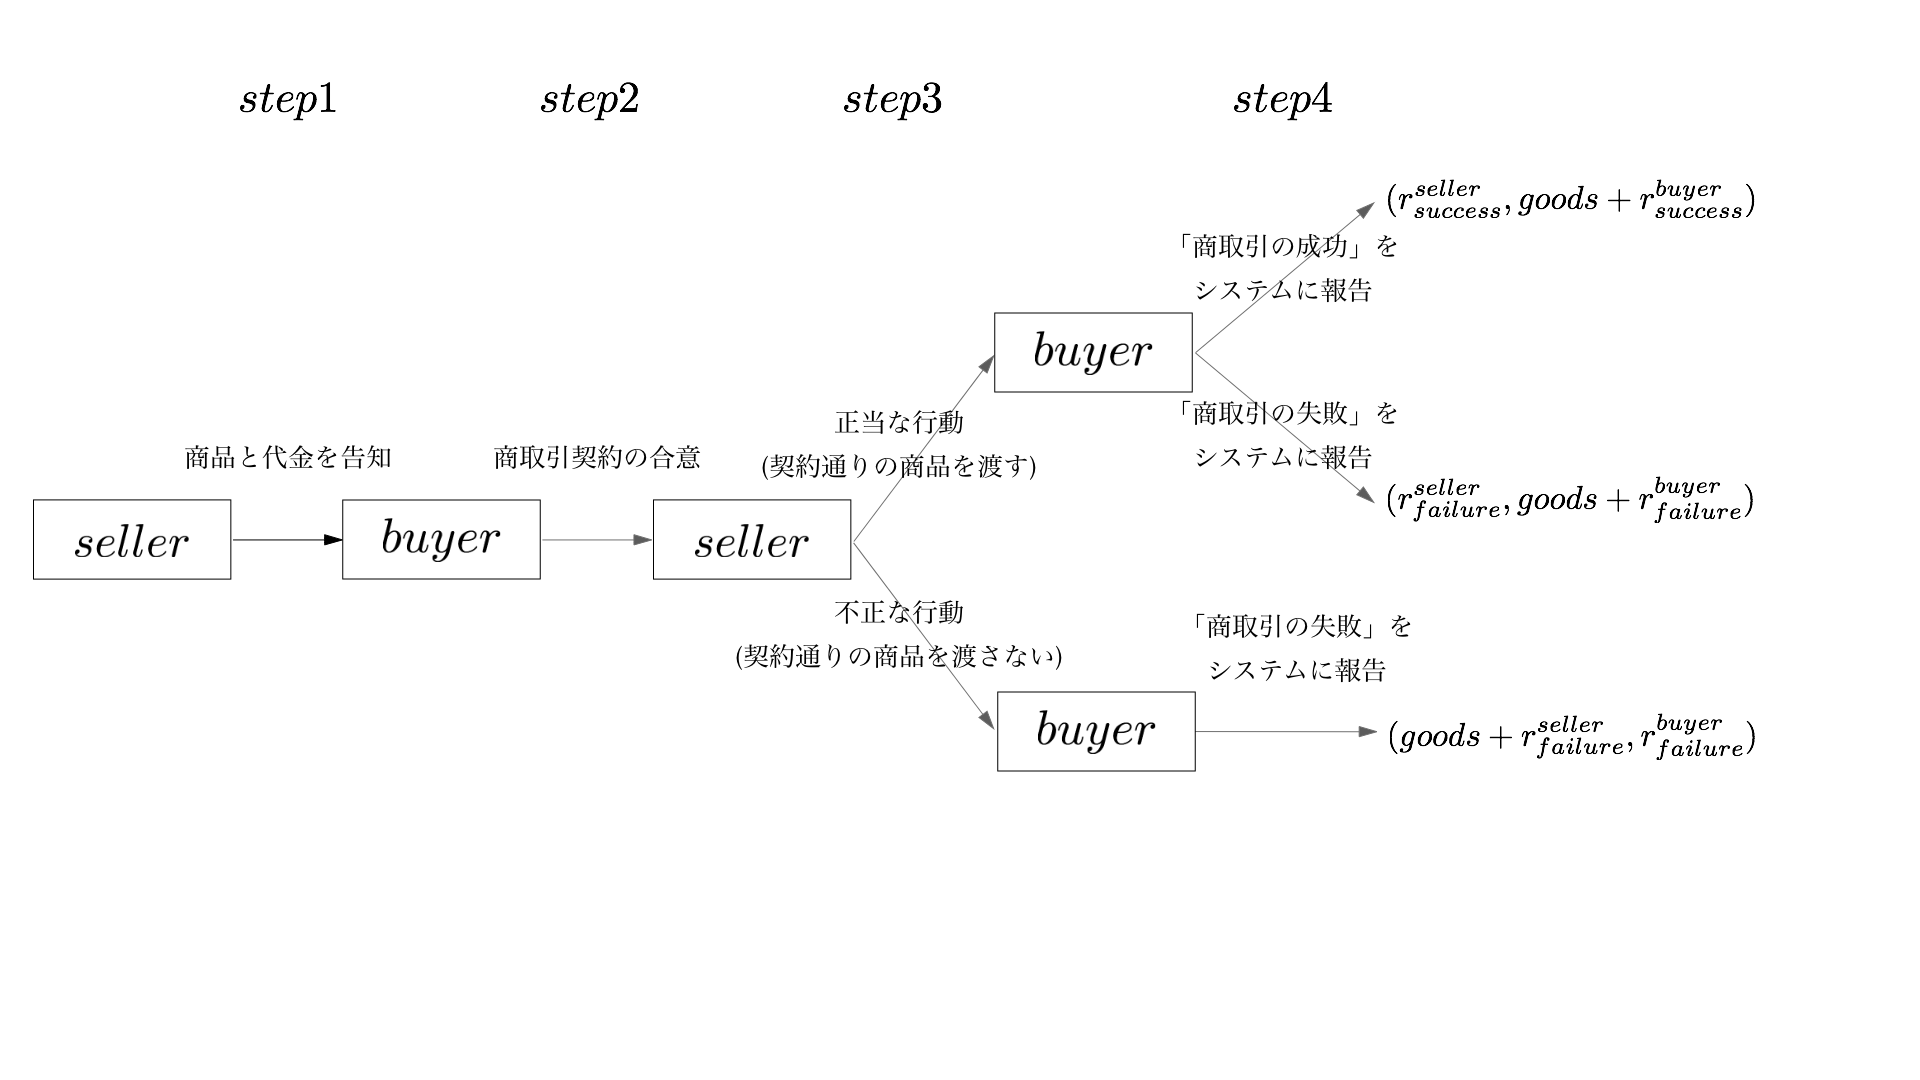
\includegraphics[width=1\linewidth]{./04_ethical-commerce-game/ethical-gametree.png}
  \caption{「倫理ある商取引ゲーム」のゲーム木}
  \label{ethical-gametree}
\end{figure*}


\begin{table*}
\centering
\begin{tabular}{|l|l|l|l|}
\hline
\multicolumn{2}{|l|}{\multirow{2}{*}{}} & \multicolumn{2}{l|}{$buyer$} \\ \cline{3-4}
\multicolumn{2}{|l|}{}                  &$s^{buyer}_1$&$s^{buyer}_3$\\ \hline
\multirow{2}{*}{$seller$}
&$s^{seller}_1$&\successseller&\fseller\\ \cline{2-4}
&$s^{seller}_2$&\fbuyer&\fbuyer\\ \hline
\end{tabular}
\caption{非協力戦略型ゲームとして表した「倫理ある商取引ゲーム」の利得表}
\label{ethical-gametable}
\end{table*}

\clearpage

\subsection{誠実な戦略が取られた割合と報告された成功率の関係}
この「倫理ある商取引ゲーム」においては,商取引が失敗した場合に必ず「失敗」が報告されるため,商取引の成功率は「商取引システム」に「成功」が報告された割合以上である.ここで任意の$ player $が任意の$ opportunity $と過去に「商取引ゲーム」を行った際,誠実な戦略($ s^{seller}_1, s^{buyer}_1 $のいずれか)をとってきた割合を$ HonestStrategyRate(player, opportunity) $とし,同様に報告された商取引の成功率を$ ReportedSuccessRate(player, opportunity) $とする.そのとき,$ HonestStrategyRate(player, opportunity) $と$ ReporttedSuccessRate(player, opportunity) $の関係は次の式で表せる.


\begin{equation}
  HonestStrategyRate(player, opportunity) \geq ReportedSuccessRate(player, opportunity)
\end{equation}

\subsection{自己信頼}
ここで$ HonestStrategyRate(player, player) $と$ ReportedSuccessRate(player, player) $は1とする.これは$ player $が$ player $自身と行う商取引は必ず成功するためである.

\subsection{将来期待利得}
通常の「商取引ゲーム」においては誠実な戦略を取ってきた割合と報告された商取引ゲームの成功率の間の関係性はわからないため,繰り返しゲームと考えても次のゲームへ引き継げる情報がなかったため将来期待利得を考慮しなかったが,「倫理ある商取引ゲーム」においては先に述べた関係式が得られるため,将来期待利得を考慮する必要がある.商取引で「成功」が報告された場合の$ seller $と$ buyer $の将来期待利得を$ \epsilon^{seller}, \epsilon^{seller} $とし,「失敗」が報告された場合の将来的な期待利得を$ \lambda^{seller}, \lambda^{buyer} $とおくと,「倫理ある商取引ゲーム」のゲーム木と非協力戦略型ゲームの表は次のように書き換えられる.
また,本稿では,これらについて$ \epsilon^{player} > \lambda^{player} $と仮定する.
